\chapter{Hybrid Beam Element Formulation}\label{chapter:CH2}


\section{Introduction}\label{section:CH2-S1}
In this chapter we present the formulation of a
novel hybrid beam element which is based on \acrshort{nlp} principles. The 
kinematic assumptions adopted fall under the category of 
geometrically exact or Simo-Reissner beam 
theory\cite{Reissner1,Simo1,Simo2,Simo3}, whereby no simplifying approximation 
is made with respect to the strain-displacement equations. This allows for 
capturing arbitrarily large displacements and rotations, as well as 
accounting for the effect of shear deformation at the section level. 

As opposed to deriving the system equations
from the Galerkin form, we recast the
problem in an \acrshort{nlp} framework by utilizing the underlying
variational structure. The total potential energy (\acrshort{tpe}) functional 
is augmented with
all relevant conditions that enforce the exact kinematics, by intoducing a set
of Lagrange multipliers that act as conjugate force quantities. The resulting
modified functional is then approximated by employing a Gauss-Legendre 
quadrature
rule, which yields the objective function to be minimized. With this particular
approach, the primary variables in the element interior contributing to the
elastic strain energy are the generalized strain measures of the
centroid, which are the unknown quantities at the quadrature points.
Displacement measures at the edge nodes of the element, namely, the translations
along coordinate axes and the rotation of cross sections, are only
associated with the external work. Kinematic consistency between the rotational
measures of displacement and strains is enforced by using a Lagrange
interpolation scheme for the curvature field, similar to the one
used by Neuenhofer and
Filippou \cite{Neuenhofer} and Schulz \& Filippou \cite{Schulz}
for force-based elements. In this work, the points used for 
the interpolation
coincide with the integration points of the quadrature rule used for 
approximating
the energy functional. To avoid ill-conditioning issues of the 
linearized operator, we also outline a block-elimination procedure for the 
linear system involving the Hessian matrix so that the
reduced system includes only displacement components. The corresponding
stiffness operator is well-conditioned, sparse, banded and symmetric. This 
renders standard \acrshort{fem} routines from existing codes 
reusable and, in conjuction with the capability for accuracy even with crude
discretization, provides an attractive formulation for fast and accurate
computation. Additionally, accuracy and locking free performance are guaranteed
with just one element per structural member, even in the presence of arbitrarily
large displacements and rotations. Accordingly, the element can also capture 
high 
curvature gradients due to plastic hinge formation, in the case of inelastic
analysis.

This chapter starts with a brief outline of the beam geometric description 
while adhering to the derivations by Cardona \& Geradin\cite{Cardona}, followed 
by the hybrid \acrshort{nlp} formulation for the element. The third section is 
devoted to implementation details, where special attention is given to the 
block 
elimination technique used for the reduction of the linear system involving the 
Hessian matrix. Finally, the chapter concludes with a set of numerical examples 
where the focus is the Hybrid \acrshort{nlp} element performance with respect 
to coarse mesh discretizations in nonlinear analysis. 

%%%%%%%%%%%%%%%%%%%%% CHAPTER 2 - SECTION 2 %%%%%%%%%%%%%%%%%%%%%%%%%%%%%%
\section{Geometrically-Exact Model}\label{section:CH2-S2}
%%%%%%%%%%%%%%%%%%%%%%%%%%%%%%%%%%%%%%%%%%%%%%%%%%%%%%%%%%%%%%%%%%%%%%%%%%

%%%%%%%%%%%%%%%%%%%%% CHAPTER 2 - SUBSECTION 1 %%%%%%%%%%%%%%%%%%%%%%%%%%%%%%
\subsection{Beam Kinematics}\label{subsection:CH2-S2SS1}
Let \{$\mathbf{E}$\} be a fixed orthonormal coordinate frame with unit vectors
$\{\bvec{E}_1,\ \bvec{E}_2,\ \bvec{E}_3\}$ along the axes $X_1, X_2, X_3$. For
an initially straight beam of length $\ell$ with its centerline coinciding with
$X_1$, the undeformed configuration is completely described by:
\begin{gather}
	\bvec{X}(X_1,X_2) = X_1\bvec{E}_1 + X_2\bvec{E}_2 =
	\bvec{r}_o(X_1)+\bvec{t}(X_2)
\end{gather}

% ADD UNDEFORMED + DEFORMED SKETCH
\begin{figure}[t]
	\centering
	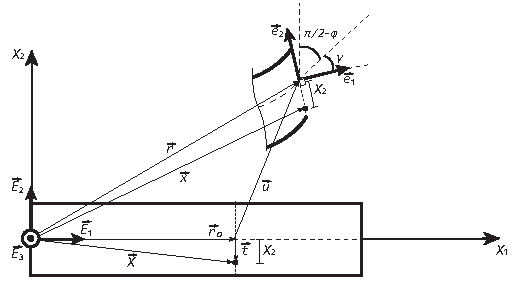
\includegraphics[scale=1.25]{FIG1_BEAM_THEORY}
	\caption{Undeformed and deformed configurations of the beam.}
	\label{fig:FIG1}
\end{figure}

\noindent where $\bvec{r}_o$ traces the centerline in the reference 
configuration
and $\bvec{t}$ locates a material point on the cross section. Assuming a
rectangular cross-section of height $h$, without loss of generality, we have 
that
$X_1\in[0,\ \ell]$ and $X_2\in[-\sfrac{h}{2}, \sfrac{h}{2}]$. We should
note here that $X_3$ is omitted as it does not explicitly come into the
expressions. We nevertheless hold on to the $\mathbb{R}^3$ vector formalism to
maintain consistency with the representation of rotation as a linear operator.
After the application of a displacement field $\bvec{u}(X_1)$, the
deformed configuration is given by vector $\bvec{x}$ such that:
\begin{gather}
	\bvec{r} = \bvec{r}_o + \bvec{u} \label{eq:def1}\\
	\bvec{x}=\bvec{r} + X_2\bvec{e}_2 \label{eq:deformed}
\end{gather}

\noindent where $\{\mathbf{e}\}$ is a local coordinate system attached at
cross-sections that completely describes their orientation. For the unit vectors
of the local base $\bvec{e}_1,\ \bvec{e}_2,\ \bvec{e}_3$, we let $\bvec{e}_1$ be
normal to the cross-section, but not necessarily tangent to the deformed
centerline, and $\bvec{e}_2$ (and $\bvec{e}_3$) coincide with the cross-section
principal axes of inertia, as shown in Fig. \ref{fig:FIG1}.

If $\bmat{R}$ is the rotation operator that rotates $\{\mathbf{E}\}$ to
$\{\mathbf{e}\}$, then:
\begin{gather}
	\bvec{e}_i = \bmat{R}\bvec{E}_i ,\quad i=1,2,3
	\label{eq:roteq}
\end{gather}

\noindent For the plane case, the component form of $\bmat{R}$ reduces to:
\begin{gather}
	\bmat{R} = \begin{bmatrix}
		\cos\phi &-\sin\phi & 0\\
		\sin\phi &\cos\phi & 0\\
		0 & 0 & 1
	\end{bmatrix}
\end{gather}

\noindent Then, using Eq. (\ref{eq:roteq}), Eq. (\ref{eq:deformed}) becomes:
\begin{gather}
	\bvec{x} = \bvec{r} + \bmat{R}\bvec{t}
	\label{eq:deformed1}
\end{gather}

\noindent For Eqs. (\ref{eq:deformed}),(\ref{eq:deformed1}) to hold in this
manner, we tacitly assume that cross-sections remain rigid during
deformation, that is, the position of a material point on a cross-section
with respect to the centroid does not change.


%%%%%%%%%%%%%%%%%%%%% CHAPTER 2 - SUBSECTION 2 %%%%%%%%%%%%%%%%%%%%%%%%%%%%%%
\subsection{Strain Measures, Strain-Displacement
Relations}\label{subsection:CH2-S2SS2}
Within the context of geometrically-exact formulations, it is common to adopt as
a strain measure $\bvec{s}$ the difference of the position vector gradients,
$\bvec{r}$ and $\bvec{r}_o$, with respect to the local frame (e.g. see
\cite{Simo1,Cardona,Hodges}). Denoting derivatives with respect to $X_1$
by $(\cdot)'$, we get:			% HERE
\begin{gather}
	\bvec{s} = \bmat{R}^T\bvec{r}'- \bvec{r}'_o
	\label{eq:strm}
\end{gather}

\noindent whereas the cross-section curvature is given as:
\begin{gather}
	\kappa=\phi'
	\label{eq:kapa}
\end{gather}

\noindent The axial and shear strain of the centroid, $\epsilon$ and
$\gamma$ respectively, can then be retained as follows:
\begin{gather}
	\epsilon = \bvec{e}_1^T\bvec{s}\\
	\gamma = \bvec{e}_2^T\bvec{s}
\end{gather}

\noindent where $\bvec{s}=\begin{bmatrix}
	\epsilon & \gamma & 0
\end{bmatrix}^T$, with the third component, representing the shear strain along
the out-of-plane axis, being by assumption zero.

Using Eq. (\ref{eq:def1}) and performing the differentiations in
Eq. (\ref{eq:strm}) with respect to $X_1$, we get:
\begin{gather}
	\bvec{s} = \bmat{R}^T[\bvec{u}'+\bvec{E}_1] - \bvec{E}_1
	\label{eq:strd}
\end{gather}

\noindent Deriving the exact differential strain-displacement relations as
presented in Reissner\footnote{See equations (15) in \cite{Reissner1}} is 
straigtforward if we solve Eq. (\ref{eq:strd}) for $\bvec{u}'$:
\begin{gather}
	\bvec{u}' = \bmat{R}\bvec{s}+\bvec{e}_1-\bvec{E}_1
	\label{eq:reissd}
\end{gather}

\noindent If we write $\bvec{u} = \begin{bmatrix} u & v & 0
\end{bmatrix}^T$, then the explicit expressions for $u',v'$ along with
Eq. (\ref{eq:kapa}) are:
\begin{subequations}
	\begin{gather}
		u'= \bvec{E}_1^T\bvec{u}'=(1+\epsilon)\cos\phi-\gamma\sin\phi-1\\
		v'= \bvec{E}_2^T\bvec{u}'=(1+\epsilon)\sin\phi+\gamma\cos\phi\\
		\phi'=\kappa\label{eq:cond3}
	\end{gather}
\end{subequations}

\noindent By introducing vectors $\bvec{d}$ and $\bvec{q}$, such that $
\bvec{d} = \begin{bmatrix}
	u & v & \phi
\end{bmatrix}^T $ and $ \bvec{q} = \begin{bmatrix}
	\epsilon & \gamma & \kappa
\end{bmatrix}^T$, we can maintain the structure of Eq. (\ref{eq:reissd}) and
express all fields involved in matrix notation, as follows:
\begin{gather}
	\bvec{d}' = \bmat{R}\bvec{q}+\bvec{e}_1-\bvec{E}_1
	\label{eq:mainsd}
\end{gather}

\noindent Strain-displacement equations as represented in Eq. (\ref{eq:mainsd})
will be subsequently utilized in the formulation of the beam model.

%%%%%%%%%%%%%%%%%%%%% CHAPTER 2 - SECTION 3 %%%%%%%%%%%%%%%%%%%%%%%%%%%%%%
\section{Nonlinear Programming Formulation of the Hybrid Beam 
Element}\label{section:CH2-S3}
%%%%%%%%%%%%%%%%%%%%%%%%%%%%%%%%%%%%%%%%%%%%%%%%%%%%%%%%%%%%%%%%%%%%%%%%%%

The hybrid beam element discretization is presented by utilizing the underlying
variational structure of the static problem. The minimizing principle for the
\acrshort{tpe} is recast here in an \acrshort{nlp}
formulation and the strain-displacement equations in (\ref{eq:mainsd}) are
incorporated, representing the equality constraints of the problem.

%%%%%%%%%%% CHAPTER 2 - SECTION 3 -S UBSECTION 1%%%%%%%%%%%%
\subsection{NLP Framework}\label{subsection:CH2-S3SS1}

The \acrshort{nlp} problem adopted herein is of the following form:
\begin{align}
	&\text{minimize} \hspace{1cm}f(\bvec{x})\nonumber\\
	&\text{subject to}\hspace{1.cm}  \bvec{h}(\bvec{x})=\bvec{0}\label{eq:nlp}\\
	&\hspace{2.4cm} \bvec{x}\in\mathcal{S}\nonumber
\end{align}

\noindent The objective function $f(\bvec{x})$ represents the total potential
energy of the structure, whereas vector $\bvec{h}(\bvec{x})$ includes the active
constraints of the program. The corresponding Lagrangian is:
\begin{gather}
	\mathcal{L}(\bvec{x},\bvec{\lambda}) = f(\bvec{x}) + 
	\bvec{\lambda}^T\bvec{h}(\bvec{x})
	\label{eq:lagr}
\end{gather}
\noindent where $\bvec{\lambda}$ are the Lagrange multipliers. The first-order
optimality conditions are given from the following expression:
\begin{gather}
	\nabla\mathcal{L}=\bvec{0}
	\label{eq:gradz}
\end{gather}

\noindent This is the standard form of a nonlinear constrained minimization
program with equality constraints, as encountered in the literature (e.g. 
\cite{Luenberger}).

%%%%%%%%%%% CHAPTER 2 - SECTION 3 -S UBSECTION 2 %%%%%%%%%%%%
\subsection{Discretization of Total Potential 
Energy}\label{subsection:CH2-S3SS2}

We consider the following decomposition of the total potential energy of a beam:
\begin{gather}
	\Pi = U - W
	\label{eq:tpe1}
\end{gather}

\noindent where $U$ and $W$ are the stored strain energy and potential energy
associated with external loading respectively. For the case of concentrated
external loads, Eq. (\ref{eq:tpe1}) can be expressed as:
\begin{gather}
	\Pi = \int_0^\ell\ \mathcal{W}_S(X_1,\bvec{q})\ dX_1 - 
	\sum_{i=1}^2\bvec{P}_i^T\bvec{u}_i
	\label{eq:tpe2}
\end{gather}

\noindent where $\mathcal{W}_S$ is the strain energy density of a cross section
at $X_1$ and $\bvec{q}$ denotes the neutral axis strain vector, 
$\bvec{P}_i$,$\bvec{u}_i$ the element nodal force and
displacement vectors, respectively. It can be proven\cite{Washizu} that for 
strain hardening materials
within the premises of small strain elastoplasticity, the exact solution to the 
problem renders $\Pi$ an absolute minimum.
Equivalently, the exact solution solves the program
in Eq. (\ref{eq:nlp}) for $f=\Pi$ with $\bvec{h}$ acting as constraints.
Assuming a stable
work-hardening material, the corresponding Euler-Lagrange equations yield the
constitutive equations of elastoplasticity (e.g. see discussion in Simo and 
Hughes
\cite{SimoHughes}). As it will be shown in subsequent sections, since the
constitutive update is carried out locally at the section fiber level.

Section stress
resultants are then given by the gradient of $\mathcal{W}_S$:
\begin{gather}
	\bvec{F}_{sec} = \nabla_{\mathbf{q}} \mathcal{W}_S
\end{gather}
with $\bvec{F}_{sec} = \begin{bmatrix} N & V & M \end{bmatrix}^T$.
\noindent In the case of linear elasticity, the energy density is
given by $\mathcal{W}_S = \frac{1}{2}[ EA\epsilon^2 + GA_s\gamma^2 +
EI\kappa^2]$  and the section resultants are:
\begin{gather*}
	\bvec{F}_{sec} = \begin{bmatrix}
		EA\epsilon\\
		GA_s\gamma\\
		EI\kappa
	\end{bmatrix}
\end{gather*}

\noindent where $A_s$ is the effective shear area of the cross-section. 
Numerical
approximation of Eq. (\ref{eq:tpe2}) by an appropriate quadrature yields:
\begin{gather}
 	\Pi(\bvec{q}_1,\ldots,\bvec{q}_n,\bvec{u}_1,\ldots\bvec{u}_N) = 
 	\sum_{i=1}^{n_q}
	w_i\mathcal{W}_{S,i} - \sum_{i=1}^2\bvec{P}^T_i\bvec{u}_i
	\label{eq:obj}
\end{gather}

\noindent with $w_i$ and $n_q$ being the weights and the number of 
integration
points respectively, and $\mathcal{W}_{S,i} = \mathcal{W}_S(\bvec{q}_i)$.
Eq. (\ref{eq:obj}) serves as the objective function of the \acrshort{nlp} of
Eq. (\ref{eq:nlp}).

%%%%%%%%%%% CHAPTER 2 - SECTION 3 - SUBSECTION 3 %%%%%%%%%%%%
\subsection{Discretization of Strain-Displacement 
Relations}\label{subsection:CH2-S3SS3}

The constrained conditions are derived by applying the same quadrature rule on
the integral form of the strain-displacement equations (\ref{eq:mainsd}):
\begin{gather}
	\bvec{d}(\ell)-\bvec{d}(0) = \int_0^\ell\ \bvec{d}'\ dX_1=\int_0^\ell\
	\bmat{R}\bvec{q}+\bvec{e}_1-\bvec{E}_1\ dX_1
	\label{eq:cintform}
\end{gather}

\noindent Using Eq. (\ref{eq:roteq}), numerical approximation of the right-hand
side integral leads to the element specific constraints:
\begin{gather}
	\bvec{h}^A = \bvec{d}(\ell)-\bvec{d}(0) - \sum_{i=1}^{n_q}
	w_i\bmat{R}_i(\bvec{q}_i+\bvec{E}_1)+\ell\bvec{E}_1=\bvec{0}
	\label{eq:dsd}
\end{gather}


\noindent The component form of Eq. (\ref{eq:dsd}) can be given as:
\begin{gather}
	\bvec{h}^A = \begin{bmatrix}
		u(\ell)-u(0) - \sum_{i=1}^{n_q} 
		w_i\bigg[(\epsilon_i+1)\cos\phi_i -
		\gamma_i\sin\phi_i\bigg] +\ell\\
		v(\ell)-v(0) - \sum_{i=1}^{n_q} 
		w_i\bigg[(\epsilon_i+1)\sin\phi_i +
		\gamma_i\cos\phi_i\bigg]\\
		\phi(\ell)-\phi(0) - \sum_{i=1}^{n_q} w_i\kappa_i
	\end{bmatrix}
\end{gather}

Although the strain fields appear explicitly
only in the weighted evaluation points of the quadrature, the rotational field
$\phi$ is involved in both the integration points and the element edge nodes.
As such, we introduce a Lagrange interpolation scheme for the curvature
field in the same fashion as in \cite{Andriotis}:
\begin{equation}
	\kappa(\xi) = \sum_{i=1}^{n_q}L_i(\xi)\kappa_i
	\label{eq:curvi}
\end{equation}

\noindent where $L_i$ are the Lagrange cardinal functions:
\begin{equation}
	L_i(\xi) = \frac{\displaystyle\prod_{j=1,j\neq i}^{n_q}
		(\xi-\xi_j)}{\displaystyle\prod_{j=1,j\neq i}^{n_q} 
		(\xi_i-\xi_j)}\text{,}\quad
	\xi=\frac{X_1}{\ell}\nonumber
\end{equation}

\noindent Substitution of Eq. (\ref{eq:curvi}) to Eq. (\ref{eq:cond3}) yields
the expression for rotations $\phi_i$:
\begin{equation}
	\phi_i-\phi(0) = \sum_{j=1}^{n_q}\bigg(\int_0^{\xi_i}L_j(x)\ 
	dx\bigg)\kappa_j =
	\sum_{i=1}^{n_q} T_{ij}\kappa_j
\end{equation}
\begin{figure*}[b]
	\centering
	\subfloat{{\includegraphics[width=7cm]{FIG2_A.pdf} }}%
	\qquad
	\subfloat{{\includegraphics[width=7cm]{FIG2_B.pdf} }}%
	\caption{Integration of curvature shape functions.}%
	\label{fig:fig2}%
\end{figure*}
\noindent with derivation of $T_{ij}$ illustrated in Fig.  \ref{fig:fig2}.
In matrix form, the above equation can be directly restated as a linear
equality constraint set as:
\begin{equation}
	\bvec{h}^B=\bvec{\phi} - \phi(0)\bvec{1} - \bmat{T}\bvec{\kappa} = \bvec{0}
	\label{eq:hb}
\end{equation}

\noindent where
\begin{gather}
	\bvec{\phi}=
	\begin{bmatrix}
		\phi_1 & \phi_2 & \cdots & \phi_{n_q}
	\end{bmatrix}^T\quad \text{,}\ \bvec{1}= \begin{bmatrix}
		1 & 1 & \cdots & 1
	\end{bmatrix}^T\in\mathbb{R}^{n_q} \nonumber\\
	\bmat{T} = L\begin{bmatrix}
		\xi_1 & \frac{\xi_1^2}{2} & \cdots & 
		\frac{\xi_1^{n_q}}{n_q}\\
		\vdots & \vdots & \ddots & \vdots\\
		\xi_{n_q} & \frac{\xi_{n_q}^2}{2} & \cdots & 
		\frac{\xi_{n_q}^{n_q}}{n_q}
	\end{bmatrix}\bmat{\Theta}^{-1}\quad \text{,}\ \bmat{\Theta} = 
	\begin{bmatrix}
		1 & \xi_1 & \xi_1^2 & \cdots & \xi_1^{n_q-1}\\
		\vdots &\vdots & \ddots & \vdots\\
		1 & \xi_{n_q} & \xi_{n_q}^2 & \cdots &\xi_{n_q}^{n_q-1}
	\end{bmatrix}\nonumber
\end{gather}

\noindent We can then collect all active constraints, Eqs.
(\ref{eq:dsd}),(\ref{eq:hb}), in one vector $\bvec{h}$:
\begin{equation}
	\bvec{h} = \begin{bmatrix}
		\bvec{h}^A \\
		\bvec{h}^B
	\end{bmatrix} = \begin{bmatrix}
		\bvec{0}\\
		\bvec{0}
	\end{bmatrix}
	\label{eq:constr}
\end{equation}

\noindent containing all constraints pertaining to one element.
While vector $\bvec{h}^A$ of strain-displacement constraints
will always contain three components for each element, the number of components 
in vector
$\bvec{h}^B$ will depend on the chosen quadrature rule.

%%%%%%%%%%% CHAPTER 2 - SECTION 3 - SUBSECTION 4 %%%%%%%%%%%%
\subsection{Lagrangian Function for the Structure}\label{subsection:CH2-S3SS4}

In order to derive the Lagrangian function in the form of Eq. (\ref{eq:lagr}),
we introduce a vector $\bvec{\lambda}$ of additional Lagrange multiplier
variables and augment Eq. (\ref{eq:obj}) with Eq. (\ref{eq:constr}):  % HERE
\begin{gather}
	\mathcal{L} = f + \bvec{\lambda}^T\bvec{h}
	\label{eq:elangr}
\end{gather}

\noindent A more convenient form for the Lagrangian function can also be
achieved by expanding $f$ into its constituents, namely, the element stored
energy and the potential energy:
\begin{gather}
	\mathcal{L} = \sum_{e=1}^{n_{el}}U^e - W +
	\bvec{\lambda}^T\bvec{h}
	\label{eq:langrT}
\end{gather}

\noindent where:
\begin{gather}
	U^e = \sum_{i=1}^{n_q} w_i\mathcal{W}_{S,i}^e \quad 
	\text{,}\quad W = 
	\sum_{i=1}^{N_{nod}}
	\bvec{P}_i^T\bvec{u}_i\nonumber
\end{gather}

\noindent where $N_{nod}$ is the total number of nodes in the 
structure. Thereby, additional elements can be simply incorporated 
by adding
their stored energy in the corresponding sum, and considering element
constraints by augmenting vectors $\bvec{\lambda}$, $\bvec{h}$, after 
transforming
them to the global system. Potential function $W$ is ``global" in the
sense that external loads and the corresponding work-conjugate displacement
degrees of freedom are directly added to the expression and are not
influenced by adding nodal contributions from adjacent elements. As a result,
no additional connectivity constraints at the element interfaces are needed,
and Eq. (\ref{eq:langrT}) is thus a global function for the
whole structure.


%%%%%%%%%%%%%%%%%%%%% CHAPTER 2 - SECTION 4 %%%%%%%%%%%%%%%%%%%%%%%%%%%%%%
\section{Implementation}\label{section:CH2-S4}
%%%%%%%%%%%%%%%%%%%%%%%%%%%%%%%%%%%%%%%%%%%%%%%%%%%%%%%%%%%%%%%%%%%%%%%%%%

The set of vectors associated with internal field variables,
$\{\bvec{y}_i\}_{i=1}^n$, is defined as $\bvec{y}_i =\begin{bmatrix}
	\bvec{q}_i & \phi_i
\end{bmatrix}^T= \begin{bmatrix}
	\epsilon_i & \gamma_i & \kappa_i & \phi_i
\end{bmatrix}^T$. Moreover, and according to Fig. \ref{fig:fig3}, we designate
the local element edge degrees of freedom in vector form as
$\bhat{d}_l = \bvec{d}(0)$ and $\bhat{d}_r = \bvec{d}(\ell)$. The element 
displacement
vector is thus $\bhat{d} = \begin{bmatrix} \bhat{d}_l^T & \bhat{d}_r^T 
\end{bmatrix}^T$. The corresponding
global displacement vector $\bvec{d}_g$ is related to the local 
vector
$\bhat{d}$ via the typical linear transformation $\bmat{\Lambda}$:  % HERE

\begin{gather}
	\bhat{d} = \begin{bmatrix}
		\bmat{\Lambda} & \bmat{0}\\
		\bmat{0} & \bmat{\Lambda}
	\end{bmatrix}\bvec{d}_g
	\quad\text{,}\quad \bmat{\Lambda}=\begin{bmatrix}
		\cos\theta & \sin\theta & 0\\
		-\sin\theta & \cos\theta & 0\\
		0 & 0 & 1
	\end{bmatrix}
\end{gather}

\begin{figure}[b]
	\centering
	\includegraphics[width=0.45\textwidth]{FIG3_ELEMENT.pdf}
	\caption{Typical element representing one member.}
	\label{fig:fig3}
\end{figure}

\noindent The element constraints of Eqs. (\ref{eq:dsd}),(\ref{eq:hb})
transformed in the global system become:  % HERE
\begin{subequations}
	\begin{gather}
		\bvec{h}^A_g = \bmat{V}_1\bvec{d}_g - 
		\bmat{\Lambda}^T\bigg[\sum_{i=1}^{n_q}
		w_i\bmat{R}_i(\bvec{q}_i+\bvec{E}_1) - \ell\bvec{E}_1\bigg]
		\label{eq:impsd1}\\
		\bvec{h}^B_g = \bvec{\phi}-\bmat{V}_2\bvec{d}_g - \bmat{T}\bvec{\kappa}
		\label{eq:impsd2}
	\end{gather}
\end{subequations}

\noindent where:
\begin{gather}
	\bmat{V}_1 = \begin{bmatrix}
		-\bmat{I} & \bmat{I}
	\end{bmatrix}\quad\text{,}\quad
	\bmat{V}_2 = \begin{bmatrix}
		\bvec{0} & \bvec{0} & \bvec{1} & \bvec{0} & \bvec{0} & \bvec{0}
	\end{bmatrix}\nonumber\\
	\bmat{I} = \begin{bmatrix}
		1 & 0 & 0\\
		0 & 1 & 0\\
		0 & 0 & 1
	\end{bmatrix}\quad\text{,}\quad 
	\bvec{0}\in\mathbb{R}^{n_q}\nonumber
\end{gather}

\noindent In the equation above the superscript denoting an element is omitted
for clarity. The element contribution to the Lagrangian of the assemblage,
denoted $\mathcal{E}^e$, is then:
\begin{gather}
	\mathcal{E}^e(\bvec{y}_1,\dots \bvec{y}_{n_q}, 
	\bvec{d}_g,\bvec{\lambda}^e) =
	U^e  + (\bvec{\lambda}^e)^T\bvec{h}^e_g
	\label{eq:implag}
\end{gather}

\noindent Notice that the external potential function $W$ is not included
in Eq. (\ref{eq:implag}) as it is added directly via the work done by external
forces in the global degrees of freedom and not from element contributions.
The element Lagrange multipliers $\bvec{\lambda}^e$ are force
conjugate measures at the corresponding degrees of freedom and $U^e$ is the
sum total of cross-section strain energies.
The Lagrangian of the whole system is accordingly given by:
\begin{gather}
	\mathcal{L}(\bvec{y}, \bvec{d}_g,\bvec{\lambda}) =
	U-W+\bvec{\lambda}^T\bvec{h}_g
	%\label{eq:globalL}
\end{gather}
\noindent which is a restatement of Eq. (\ref{eq:langrT}) in the global 
coordinate
system and $\bvec{y} = \begin{bmatrix}
	\bvec{y}_1^T & \bvec{y}_2^T & \cdots & \bvec{y}_m^T
\end{bmatrix}^T$, with $m$ being the total number of quadrature points in
the structure.

%%%%%%%%%%% CHAPTER 2 - SECTION 4 - SUBSECTION 1 %%%%%%%%%%%%
\subsection{Optimality Conditions as Structural Equilibrium Equations 
}\label{subsection:CH2-S4SS1}

In what follows, it is assumed we are dealing with quantities pertaining to
the total assemblage, after all element contributions have been resolved.
The first-order necessary optimality condition for the Lagrangian function (see 
Eq.
(\ref{eq:gradz})), after the imposition of boundary conditions, yields the
following relations:
\begin{subequations}
	\begin{gather}
		\nabla_{\mathbf{y}_i}\mathcal{L} = \nabla_{\mathbf{y}_i}U +
		[\nabla_{\mathbf{y}_i}\bvec{h}_g]\bvec{\lambda} = 
		\bvec{0}\label{eq:g1}\\
		\nabla_{\mathbf{d}_g}\mathcal{L} = -\nabla_{\mathbf{d}_g}W +
		[\nabla_{\mathbf{d}_g}\bvec{h}_g]\bvec{\lambda} = 
		\bvec{0}\label{eq:g2}\\
		\nabla_{\mathbf{\lambda}}\mathcal{L} = \bvec{h}_g = 
		\bvec{0}\label{eq:g3}
	\end{gather}\label{eq:eqtot}
\end{subequations}

\noindent Eq. (\ref{eq:g1}) expresses the equilibrium between external and
internal forces acting on the $i$-th cross-section for $i=1,2,\dots m$,
while Eq.
(\ref{eq:g2}) ensures consistency between externally applied loads and Lagrange
multipliers. Finally, Eq. (\ref{eq:g3}) requires that all constraints are
active when the minimum is attained. Explicit expressions for the first and
second derivatives of all quantities involved are given in the Appendix. We
should note that derivatives of the strain energy $U$ are computed
numerically during the \emph{cross-section state determination} phase in Sec.
(\ref{subsection:CH2-S4SS4}).

%%%%%%%%%%% CHAPTER 2 - SECTION 4 - SUBSECTION 2 %%%%%%%%%%%%
\subsection{The Hessian Matrix}\label{subsection:CH2-S4SS2}

The Hessian matrix of the Lagrangian function contains second order
information of the system and is utilized during the solution phase.
Eqs. (\ref{eq:g1})-(\ref{eq:g3}) constitute a set of nonlinear algebraic
equations and an iterative scheme is needed to solve the system. In block
matrix form, the Hessian is provided as:
\begin{gather}
	\bmat{H} = \begin{bmatrix}
		\nabla^2_{\mathbf{yy}}\mathcal{L} & \nabla^2_{\mathbf{y d_g}}\mathcal{L}
		&\nabla^2_{\mathbf{y\lambda}}\mathcal{L} \\
		\nabla^2_{\mathbf{y d_g}}\mathcal{L}^T  & 
		\nabla^2_{\mathbf{d_gd_g}}\mathcal{L} &
		\nabla^2_{\mathbf{d_g\lambda}}\mathcal{L}\\
		\nabla^2_{\mathbf{y\lambda}}\mathcal{L}^T
		&\nabla^2_{\mathbf{d_g\lambda}}\mathcal{L}^T
		&\nabla^2_{\mathbf{\lambda\lambda}}\mathcal{L}
	\end{bmatrix} = \begin{bmatrix}
		\nabla^2_{\mathbf{yy}}\mathcal{L} & \bmat{0} & 
		\nabla_{\mathbf{y}}\bvec{h}^T_g\\
		\bmat{0} & \bmat{0} & \nabla_{\mathbf{d_g}}\bvec{h}^T_g\\
		\nabla_{\mathbf{y}}\bvec{h}_g & \nabla_{\mathbf{d_g}}\bvec{h}_g & 
		\bmat{0}\\
	\end{bmatrix}
	\label{eq:hess}
\end{gather}

\noindent The resulting Hessian is fairly sparse. Moreover, the block
matrix $\nabla_{\mathbf{yy}}U$ which contains section stiffness information is
block-diagonal (see Appendix \ref{appendix:B}) and its
symmetry guarantees the full symmetry of $\bmat{H}$.

%%%%%%%%%%% CHAPTER 2 - SECTION 4 - SUBSECTION 3 %%%%%%%%%%%%
\subsection{Linearization of Equilibrium Equations}\label{subsection:CH2-S4SS3}

As mentioned in Appendix \ref{appendix:B}, the nonlinear system of equations in 
Eq.
(\ref{eq:gradz}) is solved in an incremental-iterative fashion. Linearization 
around
the current iteration $k$ yields:
\begin{gather}
	\nabla\mathcal{L}^k + \bmat{H}^k\delta\bvec{z}^k = \bvec{0}
	\label{eq:linsys}
\end{gather}
\noindent where $\bvec{z}$ is the vector of \emph{all} unknowns:
\begin{gather*}
	\bvec{z} = \begin{bmatrix}
		\bvec{y}\\
		\bvec{d}_g\\
		\bvec{\lambda}
	\end{bmatrix},\quad\text{with}\quad \bvec{y} = \begin{bmatrix}
		\bvec{y}_1\\
		\vdots\\
		\bvec{y}_m
	\end{bmatrix}
\end{gather*}
Reference to the current iteration step is omitted subsequently
for clarity.
Solving Eq. (\ref{eq:linsys}) directly may be cumbersome in
some cases, especially for problems that require denser distribution of
integration points (e.g. plasticity), since the Hessian is not banded and
may also be badly conditioned. In addition, implementation of
continuation schemes in order to attain solutions past critical points
is more involved since the state variable vector contains displacements, strains
and Lagrange multiplier unknowns. A different approach is hence sought,
where the initial linear system is reduced to a smaller one involving only the
displacement vector $\bvec{d}_g$. Restating the system in terms of its
distinct vector components $\bvec{y}$, $\bvec{d}_g$ and $\bvec{\lambda}$
gives:
\begin{gather}
	\begin{bmatrix}
		\nabla_{\mathbf{y}}\mathcal{L}\\
		\nabla_{\mathbf{d}_g}\mathcal{L}\\
		\nabla_{\mathbf{\lambda}}\mathcal{L}
	\end{bmatrix} +
	\begin{bmatrix}
		\nabla^2_{\mathbf{yy}}\mathcal{L} & \bmat{0} & 
		\nabla_{\mathbf{y}}\bvec{h}^T_g\\
		\bmat{0} & \bmat{0} & \nabla_{\mathbf{d}_g}\bvec{h}^T_g\\
		\nabla_{\mathbf{y}}\bvec{h}_g & \nabla_{\mathbf{d}_g}\bvec{h}_g & 
		\bmat{0}\\
	\end{bmatrix}\begin{bmatrix}
		\delta\bvec{y} \\ {\ }\delta\bvec{d}_g \\ \delta\bvec{\lambda}
	\end{bmatrix}
	= \begin{bmatrix}
		\bvec{0}\\ \bvec{0}\\ \bvec{0}
	\end{bmatrix}
	\label{eq:linon}
\end{gather}

\noindent Utilizing Eqs. (\ref{eq:g1})-(\ref{eq:g3}) and setting
$\delta{\bvec{\lambda}} = \bvec{\lambda}^{k+1} - \bvec{\lambda}^k$, Eq.
(\ref{eq:linon}) can be rewritten as:
\begin{gather}
	\begin{bmatrix}
		\nabla_{\mathbf{y}}U\\
		-\bvec{P}\\
		\bvec{h}_g
	\end{bmatrix} +
	\begin{bmatrix}
		\nabla^2_{\mathbf{yy}}\mathcal{L} & \bmat{0} & 
		\nabla_{\mathbf{y}}\bvec{h}^T_g\\
		\bmat{0} & \bmat{0} & \nabla_{\mathbf{d}_g}\bvec{h}^T_g\\
		\nabla_{\mathbf{y}}\bvec{h}_g & \nabla_{\mathbf{d}_g}\bvec{h}_g & 
		\bmat{0}\\
	\end{bmatrix}\begin{bmatrix}
		\delta\bvec{y} \\ {\ }\delta\bvec{d}_g \\ \bvec{\lambda}_{k+1}
	\end{bmatrix}
	= \begin{bmatrix}
		\bvec{0}\\ \bvec{0}\\ \bvec{0}
	\end{bmatrix}
	\label{eq:linprop}
\end{gather}
\noindent As mentioned previously, the gradient of the strain energy with
respect to the strain vector represents the cross-sectional
stress resultants. Solving the
first equation in the system of Eq. (\ref{eq:linprop}) for $\delta\bvec{y}$ we
get:
\begin{gather}
	\delta\bvec{y} =
	-\nabla^2_{\mathbf{yy}}\mathcal{L}^{-1}\bigg[\bvec{F}_{sec}
	+\nabla_{\mathbf{y}}\bvec{h}_g^T\bvec{\lambda}_{k+1}  \bigg]
	\label{eq:e1}
\end{gather}

\noindent Substituting Eq. (\ref{eq:e1}) in the third equation of Eq.
(\ref{eq:linprop}) and solving for $\bvec{\lambda}^{k+1}$ yields: % HERE
\begin{gather}
	\bvec{\lambda}^{k+1} = \bmat{B}^{-1}[\bvec{h}_g -
	\bvec{b}]+\bmat{B}^{-1}[\nabla_{\mathbf{d}_g}\bvec{h}_g]\delta\bvec{d}_g
	\label{eq:e3}
\end{gather}

\noindent By substituting Eq. (\ref{eq:e3}) into the second system equation
Eq.  (\ref{eq:g2}) we arrive at the familiar static equilibrium form of
the system of equations: % HERE
\begin{gather}
	\bmat{K}\delta\bvec{d}_g = \bvec{P} - \bvec{F}_{int}
	\label{eq:stiffsys}
\end{gather}

\noindent which can now be solved for the iterative displacement vector
$\delta\bvec{d}_g$. Vectors $\bvec{b}$, $\bvec{F}_{int}$ and matrices
$\bmat{B}$, $\bmat{K}$, are given by the following explicit formulas
in the global system:
\begin{subequations}
	\begin{align}
		&\bvec{b}
		=[\nabla_{\mathbf{y}}\bvec{h}_g][\nabla^2_{\mathbf{yy}}\mathcal{L}]^{-1}\bvec{F}_{sec}\label{eq:sub1}\\
		&\bvec{F}_{int} =
		[\nabla_{\mathbf{d}_g}\bvec{h}_g]^T[\bmat{B}]^{-1}[\bvec{h}_g-\bvec{b}]\label{eq:sub2}\\
		&\bmat{B}
		=[\nabla_{\mathbf{y}}\bvec{h}_g][\nabla^2_{\mathbf{yy}}\mathcal{L}]^{-1}[\nabla_{\mathbf{y}}\bvec{h}_g]^T
		 \label{eq:sub3}\\
		&\bmat{K}
		=[\nabla_{\mathbf{d}_g}\bvec{h}_g]^T[\bmat{B}]^{-1}[\nabla_{\mathbf{d}_g}\bvec{h}_g]\label{eq:sub4}
	\end{align}
\end{subequations}

\noindent where $\bvec{b}\in\mathbb{R}^p$, 
$\bvec{F}_{int}\in\mathbb{R}^{3N_{nod}}$,
$N_{nod}$ is again the number of structural nodes,
$\bmat{B}\in\mathbb{R}^{p\times p}$ with $p=m+3n_{nel}$, and
$\bmat{K}\in\mathbb{R}^{3N_{nod}\times 3N_{nod}}$. 

Equivalently, an
assembly process can also be implemented by casting 
Eqs. (\ref{eq:sub1}), (\ref{eq:sub3}) in local form, where they can be further 
simplified by being expanded in terms of element cross-section contributions:
\begin{subequations}
	\begin{align}
		\bvec{b}^e&=\sum_{i=1}^{n_q}
		[\nabla_{\mathbf{y}_i}\bvec{h}_g][\nabla^2_{\mathbf{y}_i\mathbf{y}_i}\mathcal{L}]^{-1}\bvec{F}_{sec}^{(i)}\label{eq:subb}\\
		\bmat{B}^e &= \sum_{i=1}^{n_q}
		[\nabla_{\mathbf{y}_i}\bvec{h}_g][\nabla^2_{\mathbf{y}_i\mathbf{y}_i}\mathcal{L}]^{-1}[\nabla_{\mathbf{y}_i}\bvec{h}_g]^T\label{eq:subB}
	\end{align}
\end{subequations}


\noindent where $n$ is the number of element quadrature points,
$\bvec{b}^e\in\mathbb{R}^{n_q+3}$ and 
$\bmat{B}^e\in\mathbb{R}^{(n_q+3)\times 
(n_q+3)}$. 
The element stiffness matrix $\bmat{K}^e\in\mathbb{R}^{6\times 6}$ and 
internal force vector $\bvec{F}_{int}^e\in\mathbb{R}^{6}$ are given by the same
expressions as in Eqs. (\ref{eq:sub2}), (\ref{eq:sub4}), but with the gradients
now cast in the local element form. For the assembly,
the standard \acrshort{fem} routines can be directly employed and the resulting 
global 
stiffness operator retains all properties typically associated with it in the 
context of classical finite element analysis, i.e. it is a symmetric positive 
definite matrix, it is well-conditioned and, importantly, it is sparse and
banded. Hence, in this case, the global internal force vector and the global 
stiffness matrix are given by the standard assembly process, designated here 
via operator {\large $\Lambda$}:
\begin{gather}
	\bvec{F}_{int} =\Assem_{e=1}^{n_{el}} \bvec{F}_{int}^e\label{eq:Fassemb}\\ 
	\bmat{K} = \Assem_{e=1}^{n_{el}} \bmat{K}^e
	\label{eq:assembly}
\end{gather}

with
\begin{gather}
	\bvec{F}_{int}^e =
	[\nabla_{\mathbf{d}_g}\bvec{h}_g^e]^T[\bmat{B}^e]^{-1}[\bvec{h}_{g}^e-\bvec{b}^e]\label{eq:localforce}\\
	\bmat{K}^e
	=[\nabla_{\mathbf{d}_g}\bvec{h}_g^e]^T[\bmat{B}^e]^{-1}[\nabla_{\mathbf{d}_g}\bvec{h}_g^e]
	\label{eq:localstiff}
\end{gather}

\noindent where $\bvec{h}_g^e\in\mathbb{R}^{n_q+3}$ denotes 
the \textit{element} constraint vector given by Eq. (\ref{eq:constr}) and
$\nabla_{\mathbf{d}_g}\bvec{h}_g^e\in\mathbb{R}^{(n_q+3)\times 6}$ 
its
gradient with respect to the global displacement degrees of freedom 
(\acrshort{dof}s)
associated with it, is given in Appendix \ref{appendix:A}. It is clear that 
with this formulation the inversion of large global 
matrices for
the computation of $\bmat{K}$ and $\bvec{F}_{int}$ is avoided and, instead, 
only 
inversion of the local elements flexibility matrices $\bmat{B}^e$ is required.
Given that for highly nonlinear problems we typically 
have $n\in\mathbb{N}([5,10])$ for satisfactory accuracy, this
results in an element flexibility matrix of dimension dim$(\bmat{B}^e)\leq 13$,
thus accelerating the analysis considerably. 

Having written the system of equations in the form of Eq. (\ref{eq:stiffsys}),
implementation of arc-length type schemes is now straighforward. In the
present
work, we adopt the algorithm proposed by Crisfield \cite{Crisfield3} whereby
the additional equation supplemented to the system is:
\begin{gather}
	\Delta\bvec{d}_g^T\Delta\bvec{d}_g = \Delta s^2
\end{gather}

\noindent with $\Delta s$ being the user-specified arc-length 
parameter. The
incremental displacement vector $\Delta\bvec{d}_g$ is updated in each iteration
as follows:
\begin{gather}
	\Delta\bvec{d}_g^{k} = \Delta\bvec{d}_g^{k-1} + \delta\bvec{d}_g^{k}
\end{gather}

\noindent where $k$ denotes the current iteration and
$\delta\bvec{d}_g^{k}$ is the vector of iterative displacements.

%%%%%%%%%%% CHAPTER 2 - SECTION 4 - SUBSECTION 4 %%%%%%%%%%%%
\subsubsection{Solution updating}\label{subsection:CH2-S4SS4}

After the determination, at an arbitrary iteration $k$ within
step $j$, of the iterative
displacement vector $\delta\bvec{d}_g^k$ from Eq. (\ref{eq:stiffsys}), the 
strain
and Lagrange multiplier vectors in Eqs. (\ref{eq:e1}), (\ref{eq:e3}) have
then to be updated.  The detailed steps of the updating procedure are as
described in \cref{BoxElement}.

\vspace{0.4cm}
{
\centering
\begin{Thesisbox}[label={BoxElement}]{Solution Updating.}
\noindent \textit{Step $j$, iteration $k$:} $ \begin{Bmatrix}
	\bvec{y}^0_j, & \bvec{d}^0_{g,j}, & \bvec{\lambda}^0_j, & \bvec{P}_j, &
	\Delta\bvec{y}^{k-1}_j, &
	\Delta\bvec{d}_{g,j}^{k-1}
\end{Bmatrix}$
\begin{enumerate}[start=1,label={\bfseries (\arabic*):}]
	\item Get section stiffnesses $\nabla_{\mathbf{yy}}^2\mathcal{L}^k$ from Eq.
	(\ref{eq:second}) in Appendix \ref{appendix:B} and section forces 
	$\bvec{F}_{sec}^k$ 
	from section integration, Eq. (\ref{eq:fsecx}).
	\item Evaluate $\bvec{b}^k$ and $\bmat{B}^k$ from Eqs. (\ref{eq:sub1}),
	(\ref{eq:sub3}) respectively (or, alternatively, $\bvec{b}^{e\ k}$,
	$\bmat{B}^{e\ k}$ from Eqs. (\ref{eq:subb}),
	(\ref{eq:subB})).
	\item Evaluate $\bmat{K}^k$ from Eq. (\ref{eq:sub4}), (or, alternatively,
	from Eqs. (\ref{eq:assembly}), (\ref{eq:localstiff})).
	\item Solve Eq. (\ref{eq:stiffsys}) for $\delta\bvec{d}_g^k$.
	\item Update incremental displacement vector: $\Delta\bvec{d}_{g,j}^k 
	\leftarrow
\Delta\bvec{d}_{g,j}^{k-1} +\delta\bvec{d}_g^k$.
	\item Update displacement vector: $\bvec{d}_{g,j}^k \leftarrow
	\bvec{d}_{g,j}^0 + \Delta\bvec{d}_g^k$.
	\item Update Langrange multiplier $\bvec{\lambda}_j^k$ from Eq.
	(\ref{eq:e3}).
	\item Evaluate iterative strain vector $\delta\bvec{y}^k$ from Eq.
	(\ref{eq:e1}).
	\item Update incremental strain vector: $\Delta\bvec{y}_j^k
	\leftarrow\Delta\bvec{y}_j^{k-1}+\delta\bvec{y}^k$.
	\item Update total strain vector: $\bvec{y}_{j}^k \leftarrow \bvec{y}_j^0 +
	\Delta\bvec{y}_j^k$.
	\item Evaluate $\bvec{F}_{int}^k$ from Eq. (\ref{eq:sub2}) (or,
	alternatively, from Eqs. (\ref{eq:Fassemb}), (\ref{eq:localforce})).
	\item Check $\Vert \bvec{P}_j-\bvec{F}_{int}^k\Vert \leq
	\text{tol}\cdot \Vert \bvec{P}_j-\bvec{F}_{int}^0\Vert$. 
	\item If \textbf{FALSE}, set $k\leftarrow k+1$ and go to \textbf{(1)}. If
	\textbf{TRUE}, set $j\leftarrow j+1$, $\bvec{y}^0_j\leftarrow
	\bvec{y}^k_{j-1}$, $\bvec{d}^0_{g,j}\leftarrow \bvec{d}^k_{g,j-1}$, 
	$\bvec{\lambda}^0_j\leftarrow \bvec{\lambda}^k_{j-1}$.
\end{enumerate}
\end{Thesisbox}
}
%%%%%%%%%%% CHAPTER 2 - SECTION 4 - SUBSECTION 5 %%%%%%%%%%%%
\subsection{Cross-Section State Determination}\label{subsection:CH2-S4SS5}

During the updating scheme described in the previous section, the section stress
resultants $\bvec{F}_{sec}$, along with the matrix
$\nabla_{\mathbf{yy}}^2\mathcal{L}$, are required. The latter, as seen
subsequently, corresponds to the generalized section stiffnesses. In the general
case where
inelastic behavior is considered, the stress-strain constitutive law has to be
integrated at the cross-section level and the material properties have to be
updated accordingly. In this work, each cross-section is discretized in $n_l$
number of layers and the stress update is performed independently for each 
layer.
This is equivalent to the composite midpoint rule applied along the height of
the cross-section. The shear coefficient $k_s$ is
introduced as a correction factor for the simplifying aforementioned assumption,
in accordance with Cowper \cite{Cowper}.

Below we present the kinematic and constitutive relations for a cross-section 
object. The (multiaxial) constitutive law at the fiber level is treated in the 
next chapter. The update
procedure is regarded as \emph{strain-driven}, in the sense that the known
initial state is updated given an increment in the centerline strains at a 
particular quadrature point. First, we define the stress and strain vectors 
associated with a particular fiber:

\begin{equation}
	\bvec{\sigma}_f = \begin{bmatrix}
		\sigma_{11} &  \sigma_{12}
	\end{bmatrix}^T,\quad
	\bvec{\epsilon}_f = \begin{bmatrix}
		\epsilon_{11}  & \gamma_{12}
	\end{bmatrix}^T
	\label{eq:FIBER_VECTOR_NOTATIONS}
\end{equation}

In line with the plane section hypothesis, the fiber strain vector can be 
determined from the centerline strain vector as follows:

\begin{equation}
	\begin{array}{lcl}
		\epsilon_{11} & = &\varepsilon-X_2\kappa \\
		\gamma_{12} &= &\varphi(X_2)\gamma
	\end{array}
	\Longleftrightarrow \bvec{\epsilon}_f = \bmat{N}_s\bvec{q},\quad \bmat{N}_s 
	=
	\begin{bmatrix}
		1 & 0 & -X_2\\
		0 & \varphi(X_2) & 0
	\end{bmatrix}
	\label{eq:SECTION_KIN}
\end{equation}
\noindent where $\varphi(X_2)$ is an as of now unspecified function that defines
a shear strain distribution along the height of the cross-section.

 Thus, given $\begin{Bmatrix}
	\bvec{q}, & \bvec{q}^{pl}
\end{Bmatrix}$, $\Delta\bvec{q}$, along with a set of internal state variables
(e.g. accumulated plastic strain), we can evaluate the incremental strains at
the midpoint of a layer at distance $X_2$ from the neutral axis as follows:

\begin{subequations}
	\begin{gather}
		\bvec{\epsilon}_f = \bmat{N}_s\bvec{q}\label{eq:f1}\\
		\Delta\bvec{\epsilon}_f = \bmat{N}_s\Delta\bvec{q}\label{eq:f2}
	\end{gather}
\end{subequations}

\noindent where it is reminded that $\bvec{q}$ is the vector containing the 
neutral axis generalized strains and $\bvec{\epsilon}_f$ is the strain vector
associated with the fiber midpoint. With Eqs. (\ref{eq:f1}), (\ref{eq:f2}) and
the initial state known,  we can perform the stress update which will yield the 
updated stress vector $\bvec{\sigma}_f$ and the (consistent) elastoplastic 
modulus for the fiber. The 
conjugate stress resultants associated with the assumed kinematic assumptions 
are derived from the element virtual work equation:

\begin{equation}
	\bvec{P}_l^T\delta\bvec{d}_l +\bvec{P}_r^T\delta\bvec{d}_r  = \int_V 
	\bvec{\sigma}_f^T\delta\bvec{\epsilon}_f\ 
	dV
	= \int_0^L \left[\int_A \bmat{N}_s^T\bvec{\sigma}_fdA\right]^T\bvec{q}\ dX_1
	\label{eq:VIRTUAL_WORK}
\end{equation}
where we define the conjugate section stress resultants associated with 
$\bvec{q}$ as follows:
\begin{gather}
	\bvec{F}_{sec}^{(i)}=\int_{A} \bmat{N}_s^T\bvec{\sigma}_f \ dA
	\label{eq:fsecx}
\end{gather}

\noindent Application of the composite midpoint rule on Eq. (\ref{eq:fsecx})
yields:
\begin{equation}
	\bvec{F}_{sec}^{(i)} \approx 
	\begin{bmatrix}
		\displaystyle\sum_{j=1}^{n_l} \sigma_{11,j}\Delta A_j\\
		\displaystyle\sum_{j=1}^{n_l} \sigma_{12,j} \Delta A_j\\
		\displaystyle\sum_{j=1}^{n_l} X_{2,j}\sigma_{11,j}\Delta A_j\\
	\end{bmatrix}
	\label{eq:STRESS_RES_CONJUGATE}
\end{equation}
\noindent where $\Delta A_j$ the area of layer $j$. 

Let $\bmat{C}= \partial\bvec{\sigma}_f^{}/\partial\bvec{\epsilon}_f$ designate 
the tangent modulus at a fiber. During elastic steps,
$\bmat{C}\equiv\bmat{C}^{el} = \text{diag}[E,G]$. In the next chapter we will 
see that 
during plastic steps the
diagonal components of $\bmat{C}$ are, generally, also non-zero. The tangent 
section stiffness is derived as follows:
\begin{equation}
	\bmat{k}^{(i)}_{sec} = \frac{\partial\bvec{F}_{sec}^{(i)} 
	}{\partial\bvec{q}} = 
	\int_A\bmat{N}_s^T\frac{\partial\bvec{\sigma}_f}{\partial\bvec{q}}\ dA=
	\int_A\bmat{N}_s^T\frac{\partial\bvec{\sigma}_f}{\partial\bvec{\epsilon}_f}
	\frac{\partial\bvec{\epsilon}_f}{\partial\bvec{q}}\
	dA = \int_A\bmat{N}_s^T\bmat{C}\bmat{N}_s\ dA
	\label{eq:SECTION_STIFFNESS}
\end{equation}
Application of the midpoint rule on Eq. (\ref{eq:SECTION_STIFFNESS}) yields the 
following component form for $\bmat{k}^{(i)}_s$:
\begin{equation}
	\bmat{k}^{(i)}_{sec} = \begin{bmatrix}
		C^i_{11}		& 		\varphi^iC^i_{12} & -X_2^iC^i_{11}\\
		\varphi^iC^i_{21}  &  (\varphi^i)^2C^i_{22}  &  
		-x_2^i\varphi^iC^i_{21}\\
		-X_2^iC^i_{11}  &  -x_2^i\varphi^iC^i_{12}   & (X_2^i)^2C^i_{11}
	\end{bmatrix}
	\label{eq:FIB_STIFF_CONTRIB}
\end{equation}

\noindent where $C_{ij}$ are the components of the elastoplastic consistent 
tangent modulus of the fiber. The section stiffness is then given by the 
following sum:
\begin{equation}
	\bmat{k}_{sec} = \sum_{i=1}^{n_f}\bmat{k}^{(i)}_{sec}\Delta A^i
	\label{eq:FIBER_CONTRIB_TO_STIFF}
\end{equation}

Given an increment in nodal displacements at the global/structural level, the
assembly process has to loop over all elements in order to determine the element
stiffness and internal nodal forces. This procedure, illustrated in
Fig. \ref{fig:FIG4_PROCESS}, involves analysis at three different levels: the 
global/element,
the section state determination, and the fiber stress update. Having briefly
outlined the basic theory for the hybrid element as it pertains to the first two
levels mentioned above, next we introduce the elastoplastic stress update 
formulation, which pertains to the third level of the solution process and
results in a fast return mapping algorithm.
\begin{figure}[t]
	\centering
	\includegraphics[scale=0.6]{FIG4_PROCESS}
	\caption{Solution process stages. Quantities $\bmat{K}^e$ and
		$\bvec{F}_{int}$ stand for stiffness matrix and internal nodal force 
		vector
		for element $e$ respectively.}
	\label{fig:FIG4_PROCESS}
\end{figure}

The generalized section stiffness,
$\nabla^2_{\mathbf{y}_i\mathbf{y}_i}\mathcal{L}$, is given by the second
derivatives of the Lagrangian with respect to strain vector
$\bvec{y}_i=\begin{bmatrix}
	\bvec{q}_i^T & \phi_i
\end{bmatrix}^T$:  % HERE
\begin{gather}
	\nabla^2_{\mathbf{y}_i\mathbf{y}_i}\mathcal{L} =
	\nabla^2_{\mathbf{y}_i\mathbf{y}_i}U
	+ \nabla_{\mathbf{y}_i}([\nabla_{\mathbf{y}_i}\bvec{h}_g]\bvec{\lambda})
	\label{eq:equivS}
\end{gather}

\noindent where:
\begin{gather}
	\nabla^2_{\mathbf{y}_i\mathbf{y}_i}U = w_i\begin{bmatrix}
		\bmat{k}_{sec}^{(i)} & \bmat{0}\\
		\bmat{0} & 0
	\end{bmatrix}\nonumber
\end{gather}

\noindent For the explicit expression of the second term in the right-hand side
of Eq. (\ref{eq:equivS}), see Appendix \ref{appendix:B}. It
generally includes parameters associated with section rotations and Lagrange
multipliers, and is greatly simplified if small displacement assumptions
are used.



%%%%%%%%%%%%%%%%%%%%% CHAPTER 2 - SECTION 4 %%%%%%%%%%%%%%%%%%%%%%%%%%%%%%
\section{Numerical Examples}\label{section:CH2-S5}
%%%%%%%%%%%%%%%%%%%%%%%%%%%%%%%%%%%%%%%%%%%%%%%%%%%%%%%%%%%%%%%%%%%%%%%%%%

In this section we present the capabilities and efficiency of the proposed
element in a number of well-known benchmark examples. In cases where analytical
solutions are available, they are included in the comparisons. Our results are
compared against the ones achieved i) with the structural \acrshort{fem} 
software
OpenSees\cite{OpenSees}, using its flexibility-based beam element
\cite{Neuenhofer,Neuenhofer2} with five quadrature points and fiber section
integration, and ii) with the \acrshort{fem} software Abaqus\cite{Abaqus}, using
plane-stress modeling for the frame members. For the
elastic analyses, reduced integration linear quadrilateral elements (CPS4R) were
used in Abaqus to avoid shear-locking, while for the elastoplastic
simulations, reduced integration quadratic quadrilaterals (CPS8R) elements
were used instead. For all cases the Gauss-Legendre
quadrature rule is used for approximating the integrals in Eqs.
(\ref{eq:tpe2}), (\ref{eq:cintform}). For the elastoplastic analyses, we assume
a linear isotropic hardening law and the elastoplastic modulus is given
as a percentage $r$ of the elastic modulus $E$. Moreover, we assume a
rigid rectangular cross-section shape for all cases, with shear coefficient
$k_s=0.870$\cite{Cowper}. For all examples, the SI units corresponding to
material and geometric properties are Pa and $m$, while for the load units
Newton(N) is used. The convergence termination criterion for the iterative
procedure was $10^{-7}$ for all cases. Shear deformation is
allowed to occur in all analyses unless stated otherwise.


\subsection{Cantilever with Tip Load}\label{CANTIPROB}

In this first example we demonstrate the element performance with fully 
nonlinear assumptions against available analytical solutions, 
as well as its locking-free behavior when small displacement assumptions
hold.

\subsubsection{Nonlinear analyses}
Both elastic and inelastic geometrically nonlinear cases are
considered. One
element and six integration points are used, with the beam assumed to be
inextensible, and the results are presented in Fig. 
\ref{fig:FIG5_cantielastic}. 
The elastic
case assumed $EI=10$, $L=1$ and shear-rigid response for comparison purposes 
with available exact equilibrium paths\cite{bisshopp}, while the inelastic
case allows for shear effects to take place with $GA_s=500$. In order to
maintain consistency with the attributes $EI=10$ and $L=1$, we used $E=200\times
10^9$ for Young's modulus and prescribed the height of the cross-section to be
$h=0.02$, which is now required in order to carry out the cross-sectional
stress-update.
For the material nonlinearity example, the yield stress is 
$\sigma_y=180\times10^7$ with a tangent-to-elastic modulus
ratio $r=3\%$ and results are compared against Abaqus and OpenSees. 
As can be seen in
Fig. \ref{fig:FIG5_cantielastic}, in both cases remarkable accuracy is 
achieved
with just one element. Slight differences between the Abaqus quadrilateral 
model and
the beam models are observed when extensive plastification takes place. In 
Table \ref{table:table1} we also provide distinct comparisons with exact
values for the elastic case. It is clear
that when the normalized load is equal to 1, displacements remain small, and
thus, only $n=4$ quadrature points suffice to achieve small absolute error. At
the maximum load level, however, $n=6$ quadrature points 
were required for highly accurate results. 
For the shear-rigid case exact solutions are computed from numerical evaluation 
of the
elliptic integrals that describe the problem. The reader can also consult Table
1 in \cite{Mattiasson} for a wide range of values reported. Additional results
pertaining to the elastic shear-flexible case are also reported in Table
\ref{table:table1}. For this case, we used again $GA_s=500$, $EI=10$, $L=1$ and 
compared against available 
analytical solutions from\cite{Batista2}, where the normalized load
level therein is held constant and equal to 1. The values corresponding to the
maximum normalized load equal to 10 are also reported. Although exact solutions
are not available for this load level to compare against, we can see that the 
relative
change in the transverse and axial displacement with respect to the shear-rigid
case is consistent and about $5.30\%$ and $5.40\%$,
respectively.

\begin{figure*}[t]
	\centering
	\subfloat[Elastic
	analysis]{{\includegraphics[width=6.5cm]{FIG5_cantiElastic_Review.pdf}}}%
	\qquad
	\subfloat[Inelastic
	analysis]{{\includegraphics[width=6.5cm]{FIG5_cantiPlastic_Review.pdf}}}%
	\caption{Geometrically nonlinear analyses of cantilever.}%
	\label{fig:FIG5_cantielastic}%
\end{figure*}



\begin{figure}[t]
	\centering
	\hspace*{-0.47cm}\subfloat[Elastic.]{\includegraphics[scale=0.45]{FIG6_ElasticMQN.pdf}\label{fig:elasticMQN}}\\
	\hspace*{-0.47cm}\subfloat[Inelastic.]{\includegraphics[scale=0.45]{FIG6_PlasticMQN.pdf}\label{fig:plasticMQN}}
	\caption{Moment and curvature distributions for the nonlinear 
		analyses of the cantilever.}
	\label{fig:FIG6_MQN}
\end{figure}

\begin{table*}[b]\centering
	\caption{Comparison of tip normalized displacements for different load 
	levels
		for elastic response.}
	\noindent\makebox[\textwidth]{
		\begin{tabular}{@ {}ccccccccc@ {}}\toprule[2pt]
			& & & \multicolumn{3}{c}{Shear Rigid}  & 
			\multicolumn{3}{c}{Shear Flexible}\\
			\cmidrule(r{.15em}l{.10em}){4-6} \cmidrule(r{0.15em}l){7-9}
			& $\frac{PL^2}{EI}$& $n$ & Exact & Present & Error & Exact & 
			Present & Error\\
			\midrule[0.9pt]
			\multirow{2}*{$\displaystyle\frac{\delta_2}{L}$}&$1$ & 4 & 
			0.3017207 & 0.3017206 & 1.12E-07 & 0.3178138 & 0.3178137 & 
			1.64E-07\\
			& $10$ & 6 & 0.8106090 & 0.8106113 & 2.32E-06 & - & 0.8536137 & - 
			\\
			\midrule%\addlinespace[3pt]
			\multirow{2}*{$\displaystyle\frac{L-\delta_1}{L}$}& 1 & 4 & 
			0.9435668 &
			0.9435666 & 1.82E-07 & 0.9386844 & 0.9386842 & 1.75E-07 \\
			& $10$ & 6 & 0.4450044 & 0.4450017 & 2.62E-06 & - & 0.4208910 & -\\
			\bottomrule[1.5pt]
		\end{tabular}
		
	}
	\label{table:table1}
\end{table*}

In Fig. \ref{fig:FIG6_MQN} we see how the moment and curvature
distributions change based on the beam deformations for both cases of Fig.
\ref{fig:FIG5_cantielastic}, captured at distinct
load levels. The moment values at the left fixed end are also reported on
the graphs. The observed nonlinear distributions for the elastic case are due 
to the
deformed shape of the beam being drastically different from its initial
configuration. As seen, an important feature of the formulation is its ability 
to capture curvature localization when plastic hinges are also formed. In 
displacement-based conventional beam elements, a fine mesh is in constrast 
required in the areas where plastification is expected.



\clearpage

\subsubsection{Shear-locking}
Shear locking may occur in shear deformable elements undergoing bending.
Due to inconsistent interpolation of fields that are naturally related, spurious
shear stresses develop and the element response appears to be stiffer,
particularly as the beam slenderness is increased. Appropriate numerical
treatments include using field consistent higher order elements or applying
reduced numerical integration \cite{Reddy,Prathap,ZienShear}. Here, we perform
small displacement elastic analyses for various length-to-thickness
ratios. The tip displacement ratios of $\delta_T/\delta_B$ and $\delta/\delta_B$
are then plotted against the length to thickness ratio $L/h$, where $\delta_B$
and $\delta_T$ denote the Bernoulli and Timoshenko displacements respectively.
Only one element is used with two integration points. The section dimensions
are kept fixed, while the length $L$ of the beam varies. Results, along
with used data are shown in Fig. \ref{fig:FIG7_lock}, where it can be seen 
that the
proposed element exhibits locking-free behavior.

\begin{figure}[t]
	\centering
	\includegraphics[scale=0.9]{FIG7_locking.pdf}
	\caption{Influence of $L/h$ on the tip deflection and comparison with
		analytical solution.}
	\label{fig:FIG7_lock}
\end{figure}


\subsection{Lee's Frame}
Lee's frame is a well-known benchmark for geometrically nonlinear capabilities
of beam-column element formulations.  It was first analyzed by Seng-Lip Lee
et.al. in
\cite{Lee} where the exact solution to the problem was also provided. We
first consider here the classic case, where the frame is pinned on both 
supports.
An investigation on the effect of shear flexibility to the elastic response
is also carried out by varying the length-to-thickness ratio, while maintaining
large-displacement assumptions. It is demonstrated that for ratios smaller than
five, the equilibrium path ceases to be similar to the shear-rigid case. Lastly,
we investigate the response of the same frame when both supports are fixed. This
again leads to a drastically different response, with abrupt changes in the
equilibrium path.  In all cases, the centerline is assumed inextensible.

\subsubsection{Frame with pinned supports}\label{leespinned}

An elastic, geometrically nonlinear analysis is first performed.
The minimum number of elements that can be used for this specific example is 
three
and a 4-point quadrature is applied for each element, whereas twelve flexibility
elements are required in OpenSees to achieve comparable accuracy.
For the elastoplastic analysis, again three elements are used in our
simulation with eight integration points,
whereas fourteen flexibility elements are now required in OpenSees for 
comparable
accuracy. The yield stress is $\sigma_y=1.3\times 10^{9}$ and the
tangent-to-elastic modulus \ratio is $r=3.00\%$. In the elastic
analysis, the
frame members are also considered shear-rigid, in order to remain consistent
to the initial assumptions in the original investigation\cite{Lee}.
Results are shown in Fig. \ref{fig:FIG8_LeesPinned}, with the colored
markers corresponding to the deformed profiles of the same color shown in
Fig. \ref{fig:FIG9_LeesPinnedProfiles}.

\begin{figure*}[t]
	\centering
	\subfloat[Elastic 
	analysis]{{\includegraphics[width=7.cm]{FIG8_LeesElastic.pdf}}}%
	\qquad
	\subfloat[Inelastic 
	analysis]{{\includegraphics[width=7.cm]{FIG8_LeesPlastic.pdf}}}%
	\caption{Geometrically nonlinear analyses of Lee's frame with pinned
		supports.}%
	\label{fig:FIG8_LeesPinned}%
\end{figure*}

\begin{figure*}[b]
	\centering
	\subfloat[Elastic 
	profiles]{{\includegraphics[width=6.5cm]{FIG9_ElasticProfiles.pdf} }}%
	\qquad
	\subfloat[Inelastic 
	profiles]{{\includegraphics[width=6.5cm]{FIG9_PlasticProfiles.pdf} }}%
	\caption{Deformation profiles for Lee's frame with pinned supports.}%
	\label{fig:FIG9_LeesPinnedProfiles}%
\end{figure*}
\clearpage
In Fig. \ref{fig:FIG10_shearEffectLees}, results related to shear flexibility
effects on the frame's response are shown.  As previously mentioned, in 
\cite{Lee}
the members are assumed to be shear rigid, effectively adhering to the Bernoulli
assumptions. In this example, we relax this assumption and examine how the
slenderness decrease affects the structural response. As seen in the figure,
four different length-to-thickness ratios are examined and the equilibrium
path gradually deviates from the shear-rigid case. For ratio $L/h=4$, the
equilibrium path is drastically different and the structure, after entering the
snap-back region, follows a rather complex equilibrium branch. Note that around
$\delta/L=0.5$, the structure exits its current branch and continues on a 
similar
path as in the previous cases.

\begin{figure*}[t]
	\centering
	\includegraphics[scale=1]{FIG10_ElasticLHcomp.pdf}
	\caption{Effect of shear flexibility on Lee's frame response. }
	\label{fig:FIG10_shearEffectLees}
\end{figure*}

\subsubsection{Frame with fixed supports}
This variation of the benchmark problem results in a response that exhibits
a dramatic snap-back, with abrupt changes in the stiffness sign along the
equilibrium path for the nonlinear elastic problem.
Seven integration points are used here per element and, again, one element
per member, to achieve the same accuracy as with
the Abaqus plane stress model, which terminated prematurely. 
In contrast, twenty
elements are necessary in OpenSees for comparable results. The geometric
and material properties are the same as in Sec. (\ref{leespinned}) (see Fig.
\ref{fig:FIG8_LeesPinned}). For the inelastic analysis, five integration
points are sufficient, since the response is now fairly smooth overall,
in comparison to the elastic case. All members
are shear flexible in these examples, however the contribution of shear
deformation to the overall responses is negligible for both elastic and
inelastic cases.
The response and deformation profiles for both analyses are shown in Figs.
(\ref{fig:FIG11_LeesFixed}),(\ref{fig:FIG12_LeesFixedProfiles}) respectively.

\begin{figure*}[h]
	\centering
	%\subfloat[Elastic
	%profiles]{{\includegraphics[width=5.6cm]{FixedElasticProfiles_Review.pdf} 
			%}}%
	\subfloat[Elastic
	profiles]{\includegraphics[width=6.5cm]{FIG12_FixedElasticProfiles_Review.pdf}}%
	\qquad
	\subfloat[Inelastic 
	profiles]{{\includegraphics[width=6.5cm]{FIG12_FixedPlasticProfiles.pdf} 
	}}%
	\caption{Deformation profiles for Lee's frame with fixed supports.}%
	\label{fig:FIG12_LeesFixedProfiles}%
\end{figure*}

\clearpage
\begin{figure*}[t]
	\centering
	%\subfloat[Elastic
	%analysis]{{\includegraphics[width=8.2cm]{LeesFixedElastic_Review.pdf}}}%
	\subfloat[Elastic
	analysis]{\includegraphics[width=7.cm]{FIG11_LeesFixedElastic_Review.pdf}}%
	\qquad
	\subfloat[Inelastic 
	analysis]{{\includegraphics[width=7.cm]{FIG11_LeesFixedPlastic.pdf}}}%
	\caption{Geometrically nonlinear analyses of Lee's frame with fixed
		supports.}%
	\label{fig:FIG11_LeesFixed}%
\end{figure*}

\subsection{Two-Storey Frame}

In this example a two-story frame with one bay is analyzed, first studied
regarding its plastic limit load in \cite{horne}. It was also later used as a
benchmark example by Santos \cite{Santos1}, for the performance of a nonlinear
beam finite element based on complementary energy principles. The example
is slightly modified here, however the rectangular cross-section
dimensions of the structural members and their length $L$ have been
chosen so their the slenderness remains in accordance with
\cite{Santos1}. The yield stress is $\sigma_y=0.9\times 10^6$, and the
tangent-to-elastic modulus ratio is $r=3\%$. The full frame
characteristics and discretization are shown in Fig. 
\ref{fig:FIG13_santosStruct}.

\begin{figure}[t]
	\centering
	\includegraphics[width=0.7\textwidth]{FIG13_struct.pdf}
	\caption{Two-storey portal frame discretization.}
	\label{fig:FIG13_santosStruct}
\end{figure}

The minimum number of hybrid elements for this example is eight and the number
of integration points per element for the elastic and plastic analyses are
seven and ten, respectively. For the OpenSees analyses, 36 and 48 elements
were used in total for the elastic and inelastic analyses. In both cases,
however, the OpenSees analyses stopped prematurely. Results are
demonstrated in Fig. \ref{fig:FIG14_SantosAn}, showing excellent agreement 
with
Abaqus results, while the relevant deformation profiles are
provided in Fig. \ref{fig:FIG15_SantosProfiles}.

\begin{figure*}[b]
	\centering
	\subfloat[Elastic 
	analysis]{{\includegraphics[width=7.cm]{FIG14_SantosElasticPaperFig.pdf} }}%
	\qquad
	\subfloat[Inelastic 
	anaysis]{{\includegraphics[width=7.cm]{FIG14_SantosPlasticPaperFig.pdf} }}%
	\caption{Geometrically nonlinear analyses of the two-storey frame.}%
	\label{fig:FIG14_SantosAn}%
\end{figure*}

\clearpage
\begin{figure*}
	\centering
	\subfloat[Elastic 
	profiles]{{\includegraphics[width=6.5cm]{FIG15_SantosElasticProfiles.pdf} 
	}}%
	\qquad
	\subfloat[Inelastic 
	profiles]{{\includegraphics[width=6.5cm]{FIG15_SantosPlasticProfiles.pdf} 
	}}%
	\caption{Deformation profiles for two-storey frame.}%
	\label{fig:FIG15_SantosProfiles}%
\end{figure*}


\section{Summary}
A novel geometrically exact hybrid beam element formulation is presented in 
this work,
conceptually and numerically developed using nonlinear programming principles,
instead of the traditionally used FEM techniques. Structural analysis
is accordingly seen as a nonlinear program, where the total potential energy 
functional is
treated as the objective function of the problem, constrained in the space of
feasible kinematic configurations of the structure. Field integrals in the
objective function and kinematic constraints are functions approximated by an 
appropriate quadrature rule, and
kinematics of large displacements and rotations are modeled using the exact
strain-displacement relations of Reissner's beam theory. These kinematic 
equations serve as
constraints of the nonlinear program and are appended to the objective
function by means of Lagrange multipliers. With this formulation, the
involved shear and axial strain-related fields do not need to be
interpolated, but are rather collocated 
at certain quadrature points
inside the element, as defined by the numerical integration method. The only
interpolated field is curvature, whereas displacement unknowns eventually emerge
only at element edges. A Newton-based numerical approach to the Lagrangian of
the problem is presented, based on the second-order approximation of the 
necessary
optimality conditions, and it is also appropriately connected to
standard \acrshort{fem}
assemblage techniques. Hence, using the block elimination technique, 
\acrshort{fem} assembly 
routines can be 
directly reused, while the global stiffness is assembled from the inversion of 
local
flexibility operators. This is computationally
efficient because these matrices are processed independently and their 
dimension is upper bounded, with the number of quadrature points per element
ranging from 5 to 10. The presented approach is also capable to capturing 
flexural strain localization due to plastification even when geometric 
nonlinearities are present. The efficiency of the suggested formulation is 
demonstrated through several benchmark examples and is shown to be
capable to accurately capture highly nonlinear structural behaviors with just 
one
element per member in all cases, accounting for shear flexibility and 
locking-free capabilities, while also very favorably comparing against 
well-established 
beam-column and quadrilateral finite element methodologies.